%=====================================================================
%  Vissim lab: calibration and alternative designs.  Final slides.
%
%  Figures expected in the same folder (upload to Overleaf):
%    fig_network.png      fig_sensitivity.png   fig_tradeoff.png
%    fig_residuals.png    fig_alt_network.png   fig_alt_queue.png
%    fig_alt_incident.png
%  The workflow diagram is drawn with TikZ and needs no file.
%=====================================================================
\documentclass[aspectratio=169,10pt]{beamer}

\usepackage[utf8]{inputenc}
\usepackage[T1]{fontenc}
\usepackage{lmodern}
\usepackage{booktabs}
\usepackage{graphicx}
\usepackage{tabularx}
\usepackage{xcolor}
\usepackage{tikz}
\usetikzlibrary{arrows.meta,positioning,calc}

%---------------------------------------------------------------------
% Theme
%---------------------------------------------------------------------
\definecolor{accent}{HTML}{1F5FA8}
\definecolor{lightaccent}{HTML}{E8F0FA}
\definecolor{okgreen}{HTML}{2E7D32}
\definecolor{failred}{HTML}{B3261E}
\definecolor{darktext}{HTML}{1A1A1A}

\usetheme{default}
\setbeamertemplate{navigation symbols}{}
\setbeamercolor{normal text}{fg=darktext}
\setbeamercolor{structure}{fg=accent}
\setbeamercolor{frametitle}{fg=accent}
\setbeamercolor{title}{fg=accent}
\setbeamercolor{subtitle}{fg=darktext}
\setbeamerfont{frametitle}{size=\Large,series=\bfseries}
\setbeamerfont{title}{size=\LARGE,series=\bfseries}
\setbeamertemplate{itemize item}{\color{accent}\small$\blacktriangleright$}
\setbeamertemplate{itemize subitem}{\color{accent}\scriptsize$\bullet$}
\setbeamercolor{block title}{bg=accent,fg=white}
\setbeamercolor{block body}{bg=lightaccent}
\setbeamertemplate{blocks}[rounded]

\setbeamertemplate{frametitle}{%
  \vspace{4pt}\insertframetitle\par\vspace{-2pt}
  {\color{accent}\rule{\textwidth}{0.6pt}}}
\setbeamertemplate{footline}{%
  \leavevmode\hbox{\begin{beamercolorbox}[wd=\paperwidth,ht=2.4ex,dp=1ex]{}%
  \hspace{1em}\scriptsize\color{gray}M.\,N.\ Tabassum \quad Vissim lab: calibration and alternative designs
  \hfill\insertframenumber\,/\,\inserttotalframenumber\hspace{1em}
  \end{beamercolorbox}}}

\AtBeginSection[]{%
  \begin{frame}[plain]
  \vfill
  {\color{accent}\Huge\bfseries\insertsectionhead\par}
  \vspace{6pt}{\color{accent}\rule{0.5\textwidth}{1pt}}
  \vfill
  \end{frame}}

\newcommand{\pass}{\textcolor{okgreen}{\textbf{yes}}}
\newcommand{\fail}{\textcolor{failred}{no}}
\newcommand{\hl}[1]{\textcolor{accent}{\textbf{#1}}}

%---------------------------------------------------------------------
\title{Vissim lab: calibration and alternative designs}
\subtitle{Kungsgatan and Slottsgatan, Norrk\"oping\\[2pt]
\small Automated batch simulation, Gaussian-process surrogates and scenario analysis}
\author{Muhammad Noman Tabassum}
\institute{Infra Informatics PhD course, Simulation module}
\date{October 2026}

%=====================================================================
\begin{document}
%=====================================================================

\begin{frame}[plain]
\titlepage
\end{frame}

%---------------------------------------------------------------------
\begin{frame}{Outline}
\begin{columns}[T]
\begin{column}{0.48\textwidth}
\begin{enumerate}\setlength{\itemsep}{6pt}
  \item Study site, data and model
  \item Methodology: automation and surrogates
  \item Calibration in three phases
  \item Validation and recommended model
  \item Alternative designs
  \item Conclusions and discussion
\end{enumerate}
\end{column}
\begin{column}{0.48\textwidth}
\begin{block}{Key numbers}
\small
\begin{itemize}
  \item 1\,857 calibration runs, 80 scenario runs
  \item Speed RMSE 4.53 $\rightarrow$ \hl{2.01}~km/h
  \item Tests passed 9/20 $\rightarrow$ \hl{10/20}
  \item Actuated control: delay \hl{$-26\,\%$}
\end{itemize}
\end{block}
\end{column}
\end{columns}
\end{frame}

%=====================================================================
\section{Study site, data and model}
%=====================================================================

\begin{frame}{The intersection and the field data}
\begin{columns}[T]
\begin{column}{0.50\textwidth}
\centering
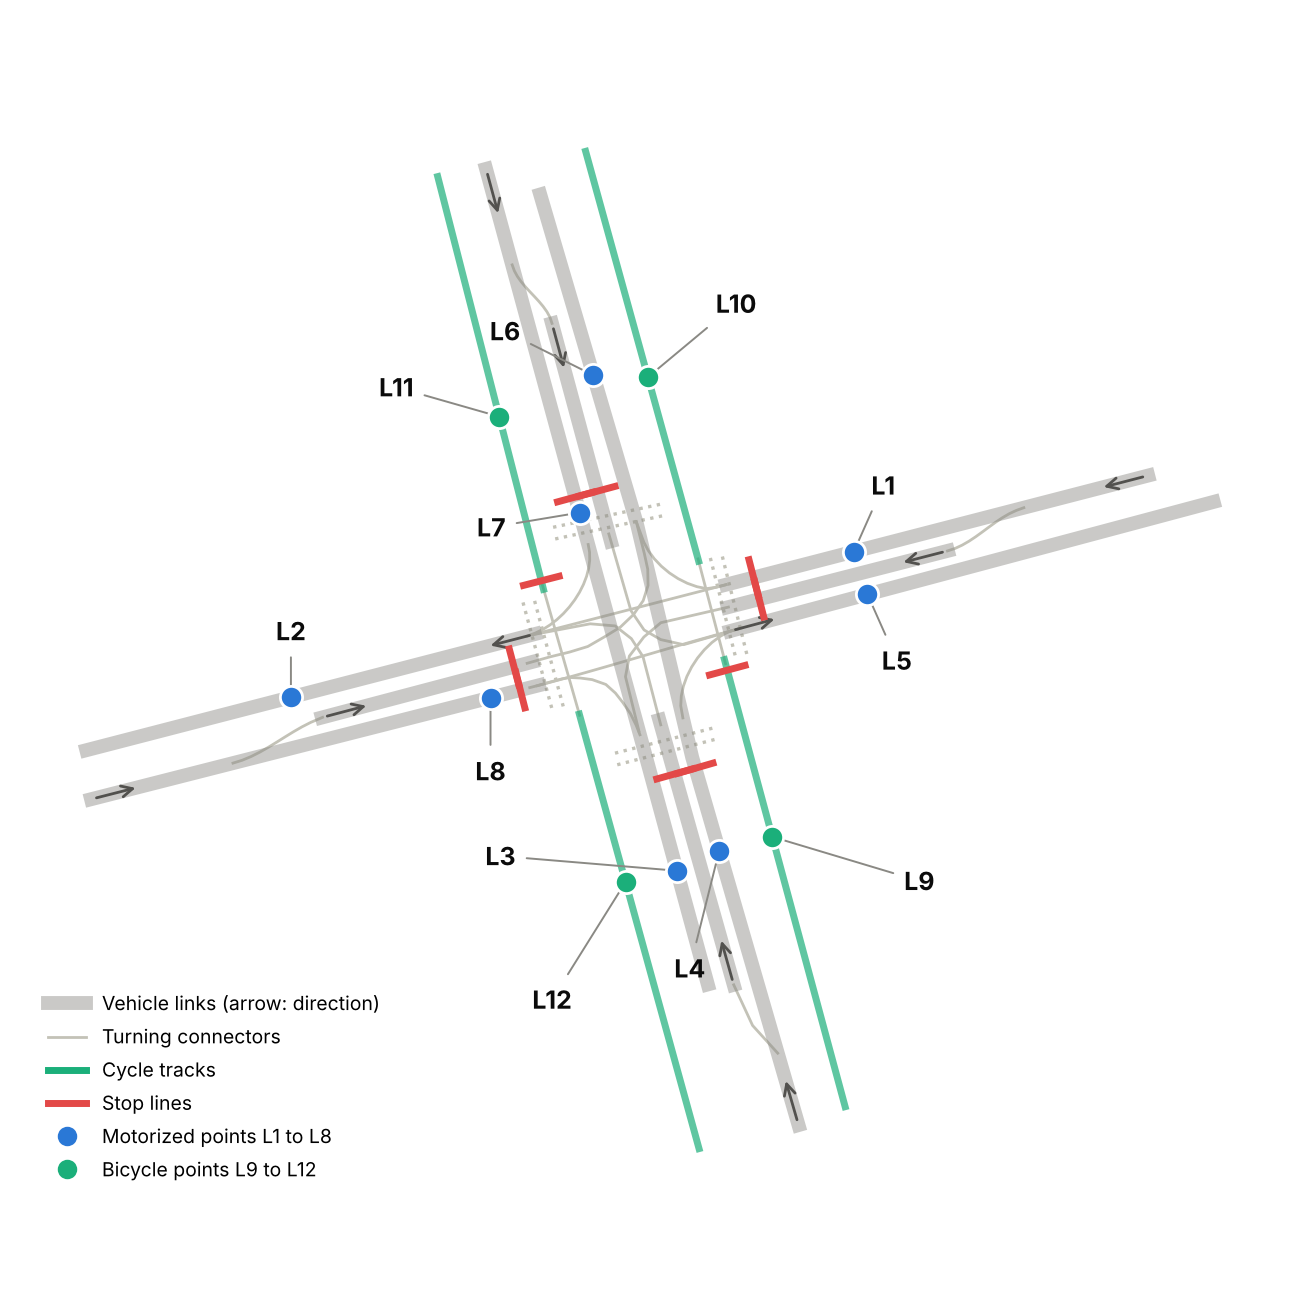
\includegraphics[width=0.92\linewidth]{fig_network.png}\\
{\scriptsize Network with the twelve measurement locations L1 to L12}
\end{column}
\begin{column}{0.48\textwidth}
\footnotesize
\begin{itemize}\setlength{\itemsep}{3pt}
  \item Four-armed signalised intersection, one lane per approach plus left-turn pockets
  \item Demand: Kungsgatan 660 and 1\,040~veh/h, Slottsgatan 240 and 210~veh/h, 100 bicycles/h per
        direction
  \item Fixed-time control, cycle 90~s: Kungsgatan about 48~s green, Slottsgatan about 38~s
  \item Kungsgatan northbound at a degree of saturation of about \hl{0.95}
  \item Field data: mean speed at L1 to L12 and mean acceleration at L1 to L8 on
        \hl{10 weekday mornings}
  \item Day-to-day s.d.\ of speed: 4.7~km/h at L1, only 0.3~km/h at L3
\end{itemize}
\end{column}
\end{columns}
\end{frame}

%---------------------------------------------------------------------
\begin{frame}{Model inventory and diagnosis}
\small
\begin{tabularx}{\textwidth}{>{\bfseries\color{accent}}p{3.2cm}X}
\toprule
Car following & Wiedemann 74: $a_x = 2.0$, $b_{x,\mathrm{add}} = 2.0$, $b_{x,\mathrm{mult}} = 3.0$,
safety-distance reduction 0.6 near stop lines\\
Desired speeds & One distribution $U(48,58)$~km/h for all inputs; compositions 4 and 5 exist but
are unused; bicycles $U(12,15)$, e-bikes $U(15,20)$\\
Acceleration & Speed-dependent desired acceleration and deceleration functions\\
Turning speeds & Right turns $U(20,25)$~km/h, but area 9 swapped; three left-turn areas without
any speed\\
Conflict areas & 91 areas, default gaps 0.5~s, safety factor 1.5\\
Evaluation & 1\,800~s from $t=0$, \hl{no warm-up} on an empty network\\
\bottomrule
\end{tabularx}
\vspace{8pt}
\begin{block}{Diagnosis of the original model (with warm-up)}
Speed RMSE 4.53~km/h, \hl{2/12} speed tests and 7/8 acceleration tests passed. Right-turners pass
L1 and L8 almost at full speed (+10.7 and +4.7~km/h); bicycles too slow ($-3.8$~km/h).
\end{block}
\end{frame}

%=====================================================================
\section{Methodology}
%=====================================================================

\begin{frame}{Surrogate-based calibration framework}
\centering
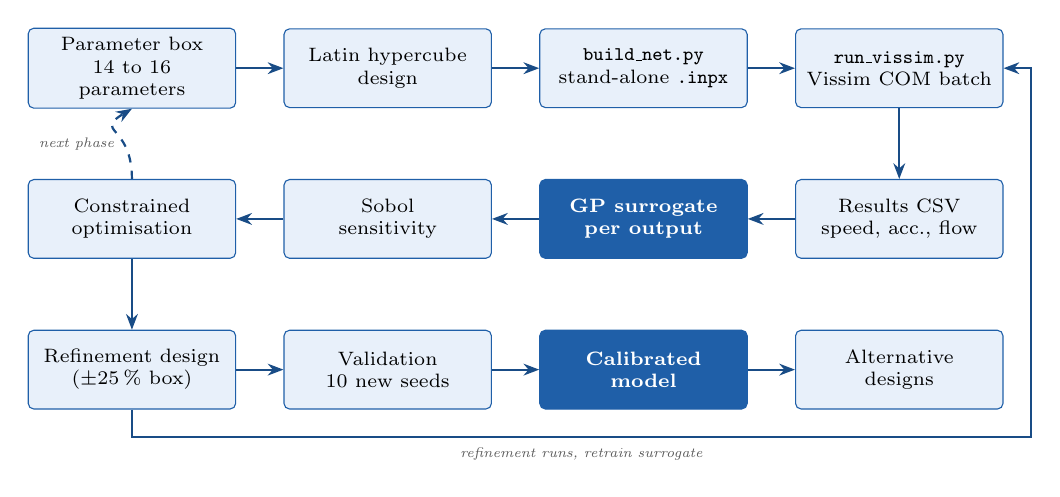
\begin{tikzpicture}[
  node distance=5mm and 6mm,
  box/.style={draw=accent, fill=lightaccent, rounded corners=2pt, align=center,
              minimum height=10mm, text width=24mm, font=\scriptsize},
  key/.style={box, fill=accent, text=white, font=\scriptsize\bfseries},
  arr/.style={-{Stealth[length=2mm]}, thick, accent!80!black},
  lab/.style={font=\tiny\itshape, text=gray!70!black}
]
\node[box] (par)   {Parameter box\\14 to 16\\parameters};
\node[box, right=of par] (lhs) {Latin hypercube\\design};
\node[box, right=of lhs] (build) {\texttt{build\_net.py}\\stand-alone \texttt{.inpx}};
\node[box, right=of build] (com) {\texttt{run\_vissim.py}\\Vissim COM batch};
\node[box, below=9mm of com] (csv) {Results CSV\\speed, acc., flow};
\node[key, left=of csv] (gp) {GP surrogate\\per output};
\node[box, left=of gp] (sobol) {Sobol\\sensitivity};
\node[box, left=of sobol] (opt) {Constrained\\optimisation};
\node[box, below=9mm of opt] (ref) {Refinement design\\($\pm 25\,\%$ box)};
\node[box, right=of ref] (val) {Validation\\10 new seeds};
\node[key, right=of val] (cal) {Calibrated\\model};
\node[box, right=of cal] (alt) {Alternative\\designs};
\draw[arr] (par) -- (lhs);
\draw[arr] (lhs) -- (build);
\draw[arr] (build) -- (com);
\draw[arr] (com) -- (csv);
\draw[arr] (csv) -- (gp);
\draw[arr] (gp) -- (sobol);
\draw[arr] (sobol) -- (opt);
\draw[arr] (opt) -- (ref);
\draw[arr] (ref) -- (val);
\draw[arr] (val) -- (cal);
\draw[arr] (cal) -- (alt);
\draw[arr] (ref.south) -- ++(0,-0.35) -| node[lab, below, pos=0.25]{refinement runs, retrain surrogate}
      ($(alt.east)+(0.35,0)$) |- (com.east);
\draw[arr, dashed] (opt.north) .. controls +(0,0.7) and +(-0.5,-0.3) .. node[lab, left, pos=0.3]{next phase} (par.south);
\end{tikzpicture}
\vspace{4pt}

\small The original \texttt{Vissim\_lab.inpx} is never modified; every variant is written as a
stand-alone network.
\end{frame}

%---------------------------------------------------------------------
\begin{frame}[fragile]{Automation: Python drives Vissim through COM}
\begin{columns}[T]
\begin{column}{0.52\textwidth}
\scriptsize
\begin{semiverbatim}
\textcolor{accent}{import} win32com.client \textcolor{accent}{as} com
vissim = com.Dispatch("Vissim.Vissim")
vissim.LoadNet(r"C:\textbackslash{}Temp\textbackslash{}variant.inpx", False)
sim = vissim.Simulation
sim.SetAttValue("NumRuns", 10)
sim.SetAttValue("RandSeed", 1001)
sim.SetAttValue("RandSeedIncr", 7)
vissim.SuspendUpdateGUI()
sim.RunContinuous()
vissim.ResumeUpdateGUI()
\textcolor{accent}{for} m \textcolor{accent}{in} vissim.Net.DataCollectionMeasurements.GetAll():
    v = m.AttValue("SpeedAvgArith(1,1,All)")
    a = m.AttValue("Acceleration(1,1,All)")
\end{semiverbatim}
\end{column}
\begin{column}{0.46\textwidth}
\small
\begin{itemize}\setlength{\itemsep}{4pt}
  \item \texttt{build\_net.py}: edits the XML (driving behaviour, speed distributions,
        compositions, acc./dec.\ functions, turning speeds, warm-up)
  \item \texttt{run\_vissim.py}: batch runs in quick mode, resumable, reads all replications
  \item \texttt{analyse.py}: statistics, GP, Sobol, optimisation, reports
  \item Fixed obstacle: scenario-management network $\rightarrow$
        \texttt{underScenMngm="false"}
  \item About 21~s per configuration with 3 runs
\end{itemize}
\end{column}
\end{columns}
\end{frame}

%---------------------------------------------------------------------
\begin{frame}{Statistical setup}
\begin{columns}[T]
\begin{column}{0.5\textwidth}
\small
\textbf{Simulation settings}
\begin{itemize}
  \item 600~s warm-up + 1\,800~s evaluation
  \item Calibration: 3 runs, common random numbers
  \item Validation: 10 runs, independent seeds
\end{itemize}
\vspace{4pt}
\textbf{Acceptance}: course $t$-test per location
\[
T = \frac{\bar x - \bar y}{\sqrt{s_p^2\,(1/n_x + 1/n_y)}},\quad |T| < 2.101
\]
\textbf{Replications}: $n = \left(t\,s_x/(\varepsilon\,\bar x)\right)^2$, $\varepsilon = 5\,\%$
\end{column}
\begin{column}{0.48\textwidth}
\small
\textbf{Surrogate}: one Gaussian process per output, Mat\'ern 5/2 with one length scale per
parameter plus white noise; 5-fold cross-validation\\[4pt]
\textbf{Sensitivity}: total Sobol indices (Saltelli, Jansen)\\[4pt]
\textbf{Optimisation}: $2^{15}$ Sobol points + elite local search\\[4pt]
\textbf{Realism constraints}
\begin{itemize}
  \item $\mathrm{GEH} \le 5$ at L1 to L8
  \item served flow at L4 $\ge 0.97\times$ original
\end{itemize}
\end{column}
\end{columns}
\end{frame}

%=====================================================================
\section{Calibration in three phases}
%=====================================================================

\begin{frame}{Three phases: what changed and why}
\small
\begin{tabularx}{\textwidth}{cccX}
\toprule
\textbf{Phase} & \textbf{Parameters} & \textbf{Runs} & \textbf{Objective and main idea}\\
\midrule
1 & 15 & 659 & Speed RMSE; broad screening of all candidate mechanisms\\
2 & 14 & 659 & $\mathrm{RMSE}_v/s_v + \mathrm{RMSE}_a/s_a$; desired speed per input\\
3 & 16 & 539 & Hinge loss in units of the $t$-test; shape of acceleration function, separate
right-turn speeds; 404 earlier configurations reused\\
\bottomrule
\end{tabularx}
\vspace{10pt}
\begin{columns}[T]
\begin{column}{0.48\textwidth}
\begin{block}{Phase 1 lesson}
Speed RMSE 1.34~km/h, but deceleration at its lower bound: acceleration RMSE 0.11 $\rightarrow$
0.53~m/s$^2$. \hl{Right for the wrong reason.}
\end{block}
\end{column}
\begin{column}{0.48\textwidth}
\begin{block}{Phase 3 lesson}
More freedom gives no more passed tests; parameters drift to implausible bounds. Remaining errors are
\hl{structural}.
\end{block}
\end{column}
\end{columns}
\end{frame}

%---------------------------------------------------------------------
\begin{frame}{Which parameters matter? Global sensitivity}
\begin{columns}[c]
\begin{column}{0.60\textwidth}
\centering
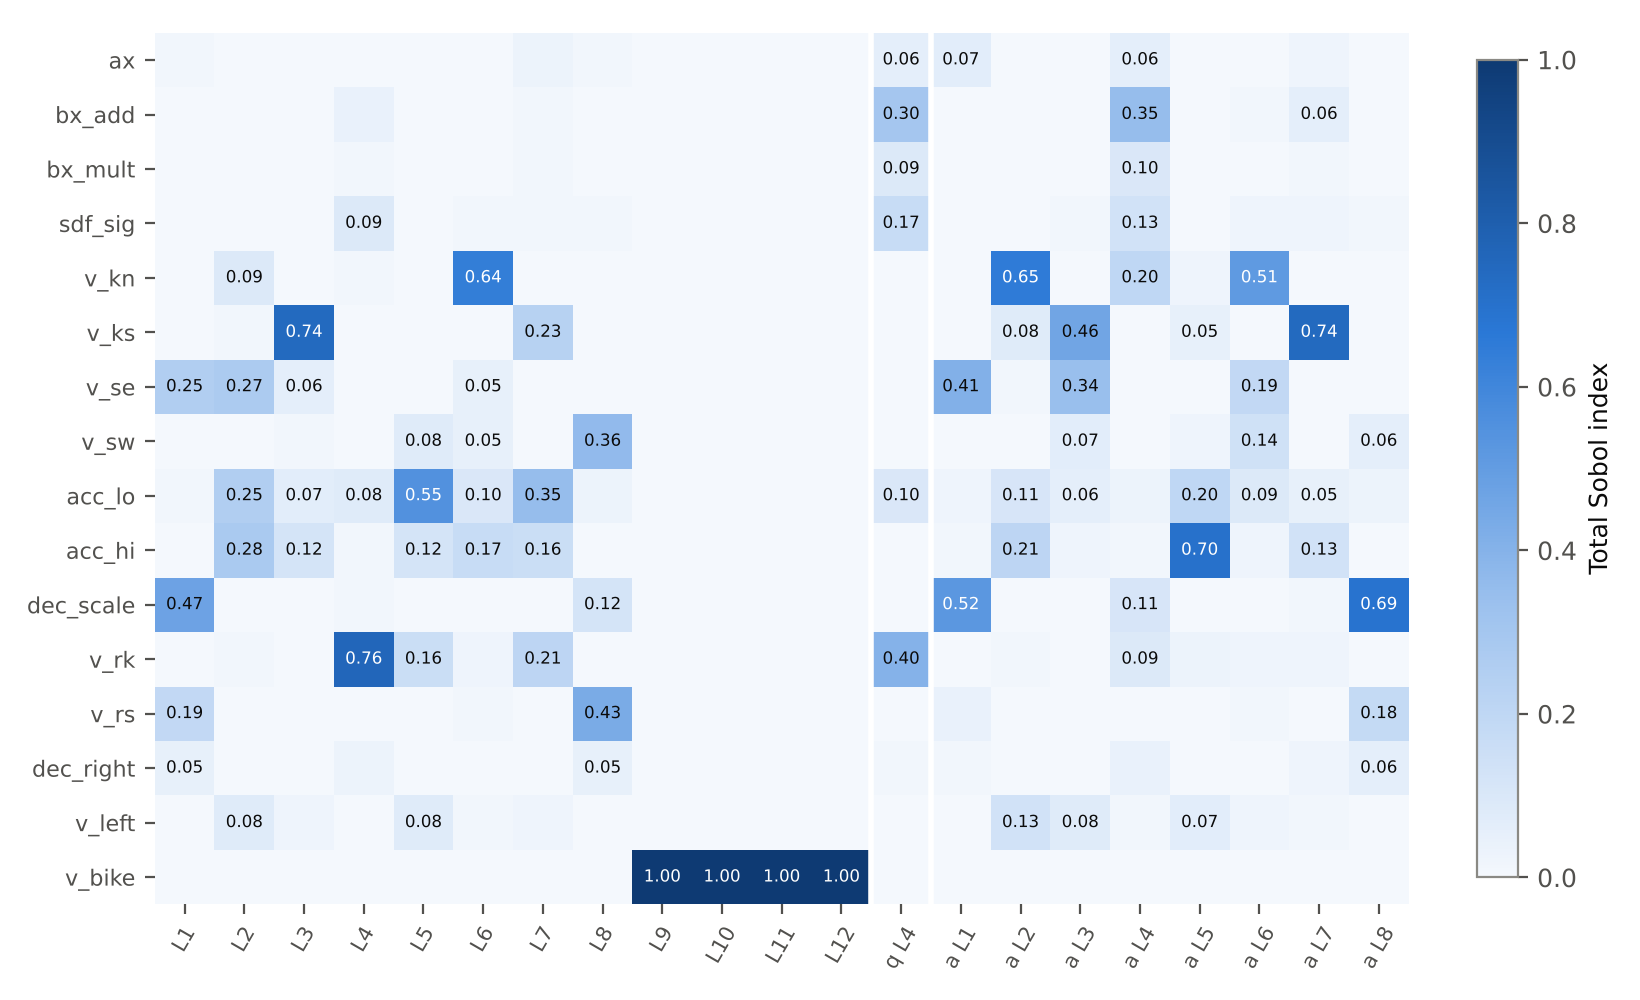
\includegraphics[width=\textwidth]{fig_sensitivity.png}\\
{\scriptsize Total Sobol indices, phase-3 surrogate (567 configurations)}
\end{column}
\begin{column}{0.38\textwidth}
\small
\begin{itemize}\setlength{\itemsep}{4pt}
  \item Right-turn speed: L4 ($S_T = 0.76$), L8, L1
  \item Desired speed per approach: exits L2, L3, L5, L6
  \item Acceleration shape: L5, L7
  \item Deceleration: L1
  \item Bicycle desired speed: L9 to L12 ($S_T \approx 0.97$)
  \item Conflict-area gaps: \hl{no influence}
\end{itemize}
\vspace{4pt}
{\scriptsize Surrogate accuracy: cross-validated $R^2 \ge 0.976$ for all speeds}
\end{column}
\end{columns}
\end{frame}

%---------------------------------------------------------------------
\begin{frame}{Speed versus acceleration: a structural trade-off}
\begin{columns}[c]
\begin{column}{0.52\textwidth}
\centering
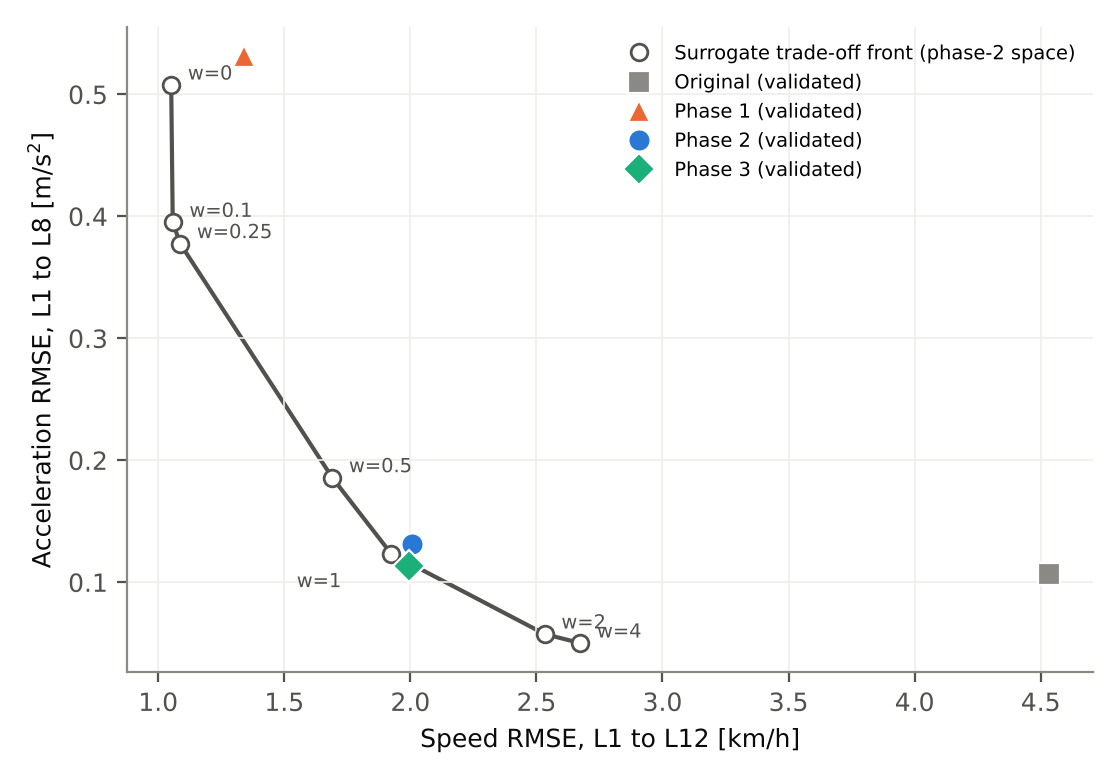
\includegraphics[width=\textwidth]{fig_tradeoff.png}\\
{\scriptsize Surrogate optima for increasing acceleration weight $w$; markers: validated models}
\end{column}
\begin{column}{0.46\textwidth}
\small
\begin{itemize}\setlength{\itemsep}{5pt}
  \item Below a speed RMSE of about 1.9~km/h the acceleration error rises sharply
  \item The conflict comes almost entirely from \hl{L1}
  \item Low field speed (17.5~km/h) needs gentle braking; strong field deceleration
        ($-1.79$~m/s$^2$) needs firm braking
  \item The model cannot do both: right-turners slow down only after the stop line
\end{itemize}
\end{column}
\end{columns}
\end{frame}

%=====================================================================
\section{Validation and recommended model}
%=====================================================================

\begin{frame}{Validation with 10 independent seeds}
\centering
\small
\begin{tabular}{lrrrr}
\toprule
 & \textbf{Original} & \textbf{Phase 1} & \textbf{Phase 2} & \textbf{Phase 3}\\
\midrule
Calibration target & & speeds & speeds + acc. & $t$-test based\\
\midrule
Speed RMSE [km/h] & 4.53 & \textbf{1.34} & 2.01 & 2.00\\
Acceleration RMSE [m/s$^2$] & \textbf{0.107} & 0.531 & 0.131 & 0.114\\
Speed tests passed & 2/12 & 6/12 & \textbf{7/12} & \textbf{7/12}\\
Acceleration tests passed & \textbf{7/8} & 1/8 & 3/8 & 2/8\\
All tests passed & 9/20 & 7/20 & \textbf{10/20} & 9/20\\
Speed RMSE, odd / even days & 4.48 / 4.63 & 1.28 / 1.55 & 1.83 / 2.27 & 1.95 / 2.14\\
Maximum GEH & 0.68 & 0.68 & 0.68 & 0.69\\
\bottomrule
\end{tabular}
\vspace{10pt}
\begin{block}{Recommendation}
\hl{Phase 2}: halves the speed error, keeps the acceleration profile, passes the most tests, serves
the demand and holds on odd and even field days.
\end{block}
\end{frame}

%---------------------------------------------------------------------
\begin{frame}{Residuals per location}
\centering
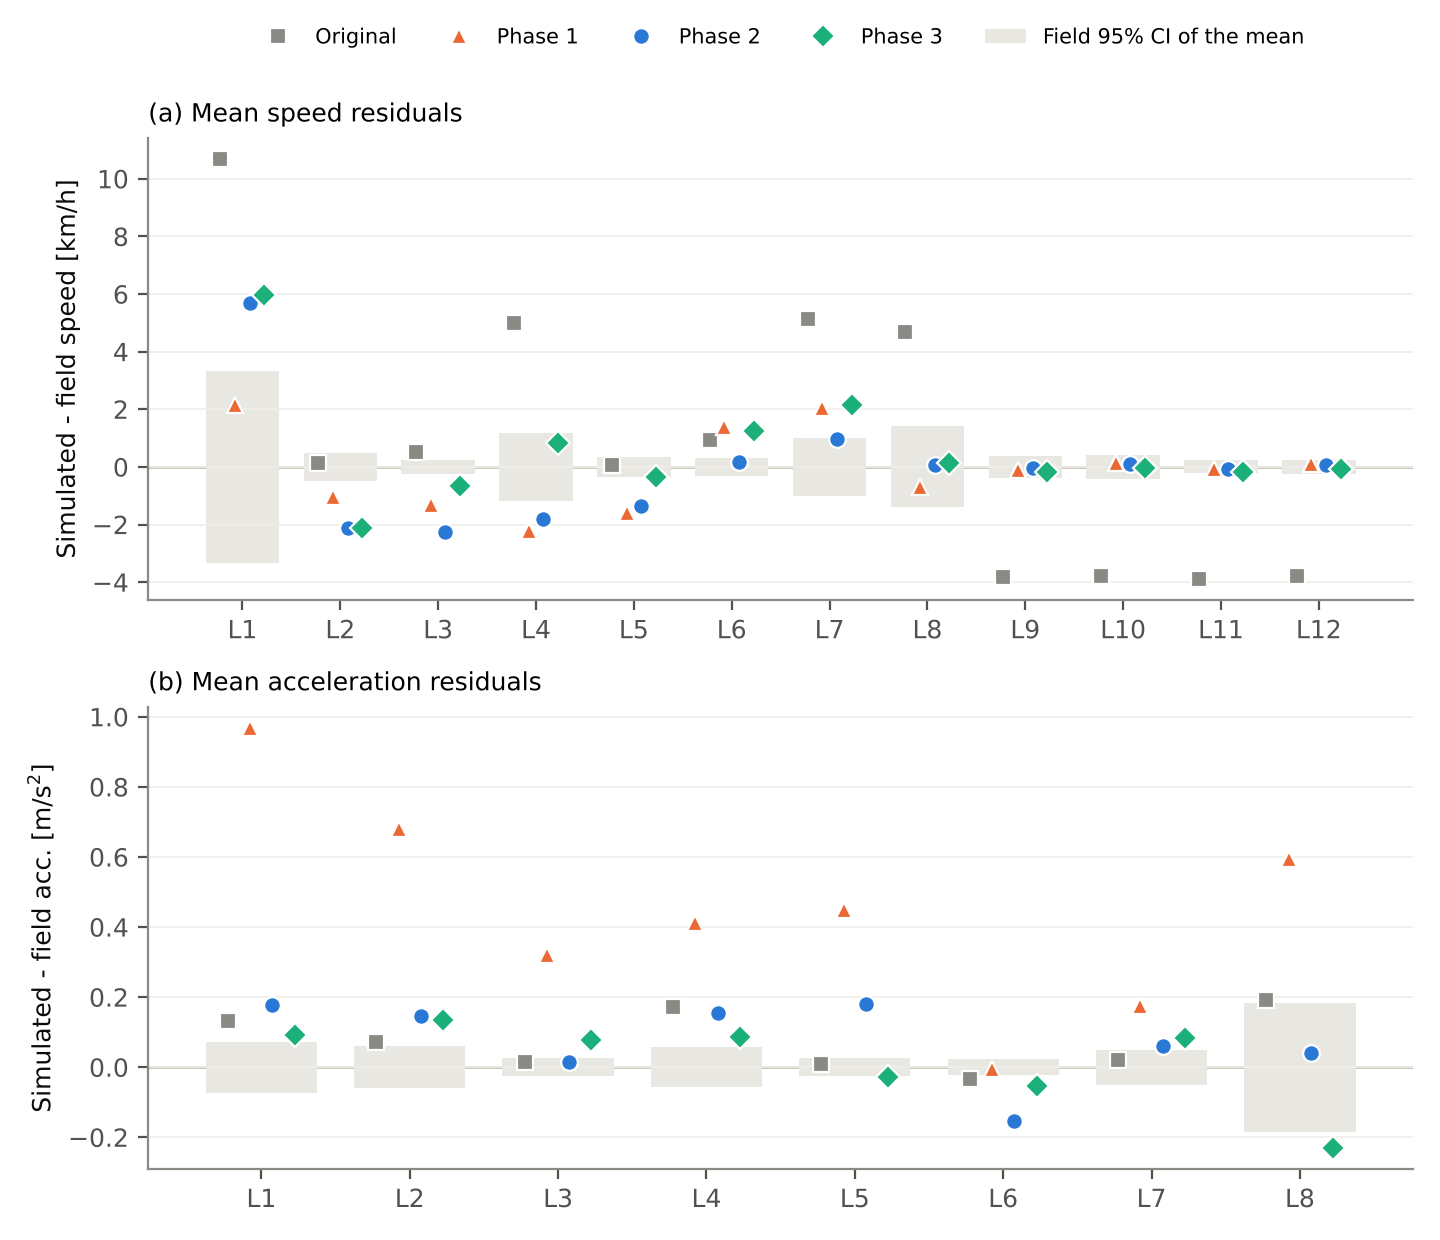
\includegraphics[height=0.74\textheight]{fig_residuals.png}\\
{\scriptsize Simulated minus field mean (10 new seeds); grey bars: 95\,\% confidence interval of
the field mean}
\end{frame}

%---------------------------------------------------------------------
\begin{frame}{Calibrated parameters (phase 2) and their meaning}
\begin{columns}[T]
\begin{column}{0.50\textwidth}
\footnotesize
\resizebox{\linewidth}{!}{%
\begin{tabular}{lrr}
\toprule
\textbf{Parameter} & \textbf{Original} & \textbf{Phase 2}\\
\midrule
$a_x$ [m] & 2.00 & 1.49\\
$b_{x,\mathrm{add}}$ / $b_{x,\mathrm{mult}}$ & 2.00 / 3.00 & 0.82 / 1.39\\
Safety reduction near signal & 0.60 & 0.31\\
Desired speed Kungsg.\ N / S & 53 / 53 & 51.7 / 51.3\\
Desired speed Slottsg.\ E / W & 53 / 53 & 43.9 / 52.4\\
Acc.\ / dec.\ scale & 1.00 / 1.00 & 1.04 / 0.89\\
Right-turn speed [km/h] & 22.5 & 10.1\\
Left-turn speed [km/h] & (27.5) & 29.9\\
Bicycle / e-bike [km/h] & 13.5 / 17.5 & 17.3 / 21.3\\
\bottomrule
\end{tabular}}
\end{column}
\begin{column}{0.47\textwidth}
\small
\begin{itemize}\setlength{\itemsep}{5pt}
  \item \hl{Bicycles} about 17~km/h: removes the 3.8~km/h bias
  \item \hl{Right turns} about 10~km/h: lowers approach speeds at L1, L4, L8
  \item \hl{Slottsgatan east} slower than the other streets
  \item \hl{Tighter car following} keeps the near-saturated approach at capacity
  \item 10 to 14 replications needed at L1 and L8 ($\varepsilon = 5\,\%$)
\end{itemize}
\end{column}
\end{columns}
\end{frame}

%=====================================================================
\section{Alternative designs}
%=====================================================================

\begin{frame}{Scenarios and experimental setup}
\small
Baseline = calibrated model (phase 2), fixed time, constant demand, 100 bicycles/h.
\vspace{6pt}
\begin{itemize}\setlength{\itemsep}{6pt}
  \item \hl{Actuated control}: VisVAP logic, gap 3~s on the detectors; stage 1 (Kungsgatan) up to
        75~s, stage 2 (Slottsgatan) up to 15~s
  \item \hl{Incident}: inputs A, C, E, G change every 10 min (Table 1 of the lab); 30-min
        averages equal the baseline, so only the \emph{timing} of demand changes
  \item \hl{800 bicycles/h} per direction instead of 100
\end{itemize}
\vspace{6pt}
\begin{columns}[T]
\begin{column}{0.48\textwidth}
\begin{block}{Design of the experiment}
20 replications per scenario with \textbf{common random numbers} $\rightarrow$ paired $t$-tests
\end{block}
\end{column}
\begin{column}{0.48\textwidth}
\begin{block}{Metrics}
Delay and stops per vehicle, queue length per approach in 10-min intervals, speeds and flows at
L1 to L12
\end{block}
\end{column}
\end{columns}
\end{frame}

%---------------------------------------------------------------------
\begin{frame}{Network performance}
\centering
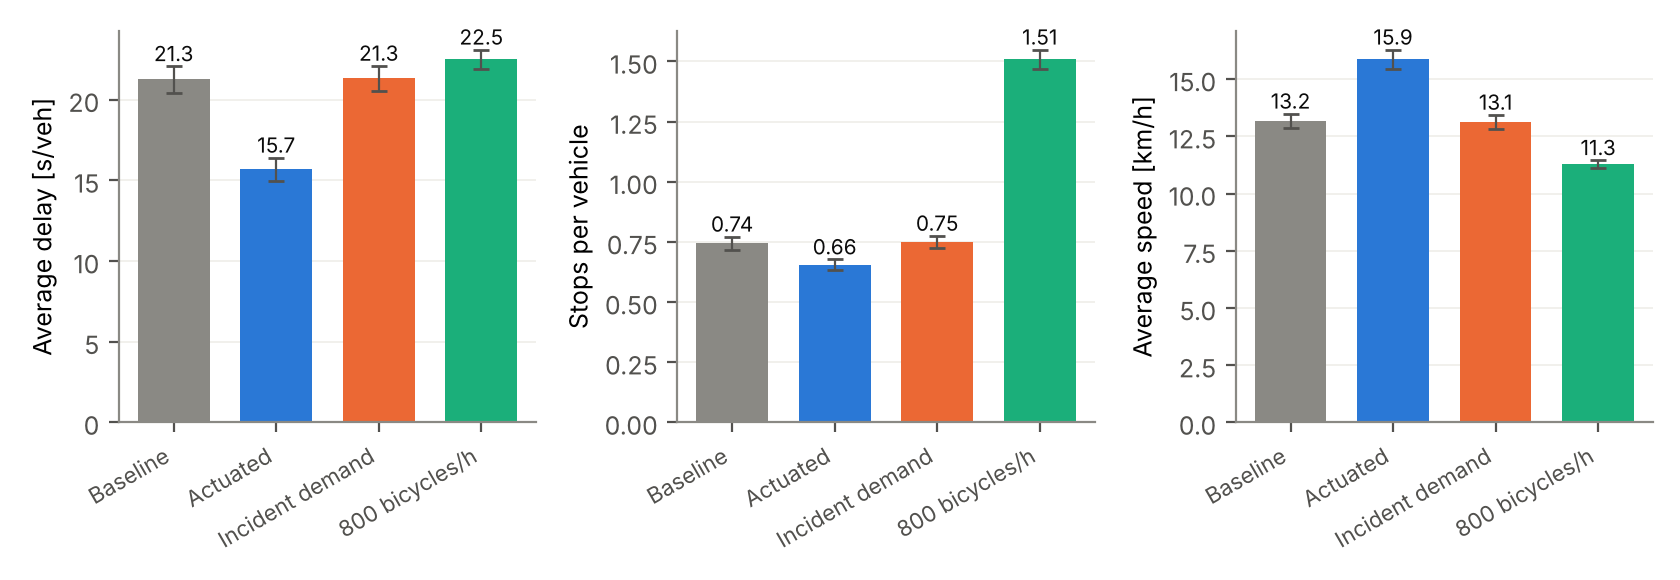
\includegraphics[height=0.52\textheight]{fig_alt_network.png}\\[4pt]
\footnotesize
\setlength{\tabcolsep}{4pt}
\begin{tabular}{lcccc}
\toprule
 & \textbf{Baseline} & \textbf{Actuated} & \textbf{Incident} & \textbf{800 bikes/h}\\
\midrule
Delay [s/veh] & 21.3 & \textbf{15.7} & 21.3 & 22.5\\
$\Delta$ delay, paired $t$-test & & $-5.6$ ($p<0.001$) & $+0.1$ ($p=0.67$) & $+1.2$ ($p<0.001$)\\
Stops [1/veh] & 0.74 & 0.66 & 0.75 & 1.51\\
\bottomrule
\end{tabular}
\end{frame}

%---------------------------------------------------------------------
\begin{frame}{Where the queues are}
\centering
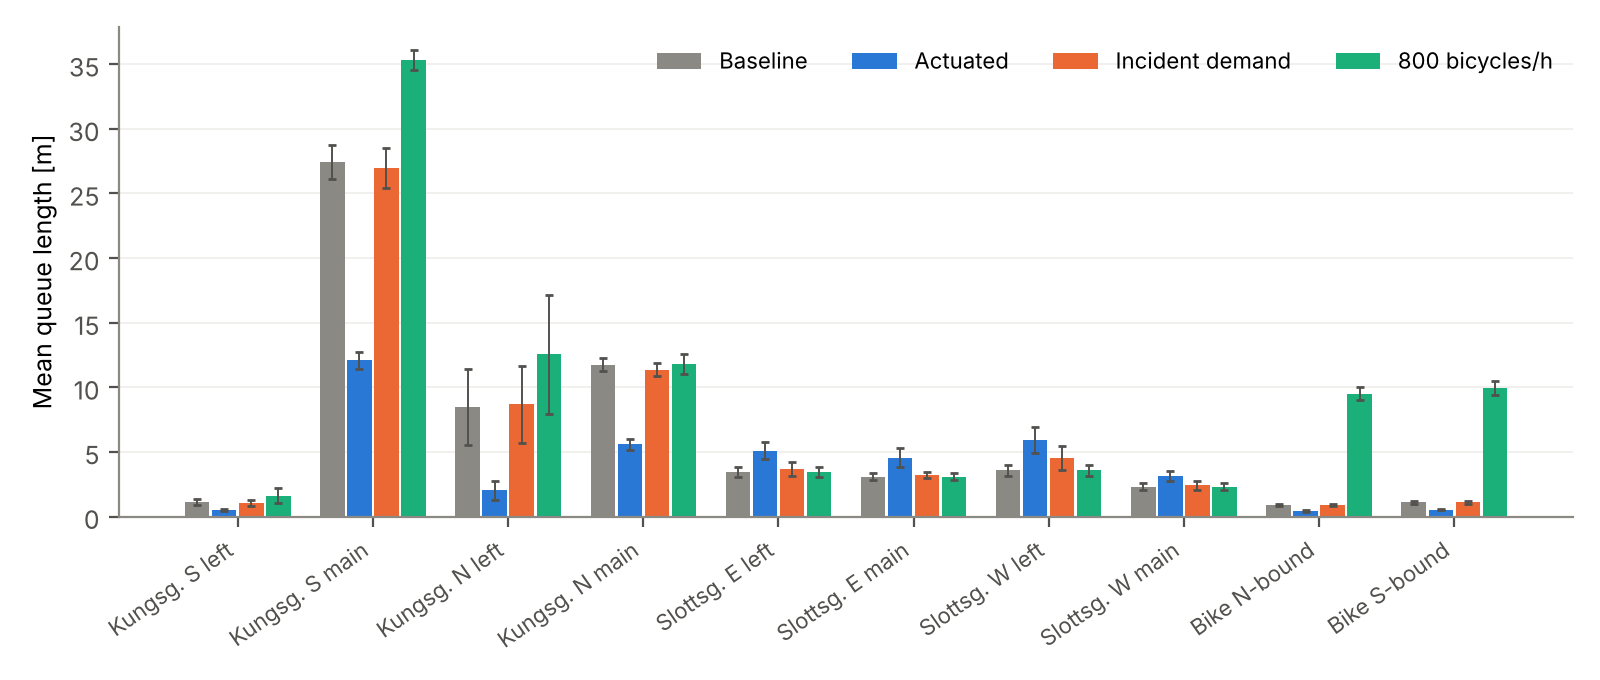
\includegraphics[width=0.85\textwidth]{fig_alt_queue.png}\\[4pt]
\small
Actuated control: Kungsgatan northbound queue \hl{27.5 $\rightarrow$ 12.1~m}, southbound
11.8 $\rightarrow$ 5.6~m; Slottsgatan queues grow by 1 to 2~m.\\
800 bicycles/h: northbound queue 27.5 $\rightarrow$ 35.3~m.
\end{frame}

%---------------------------------------------------------------------
\begin{frame}{Incident dynamics}
\centering
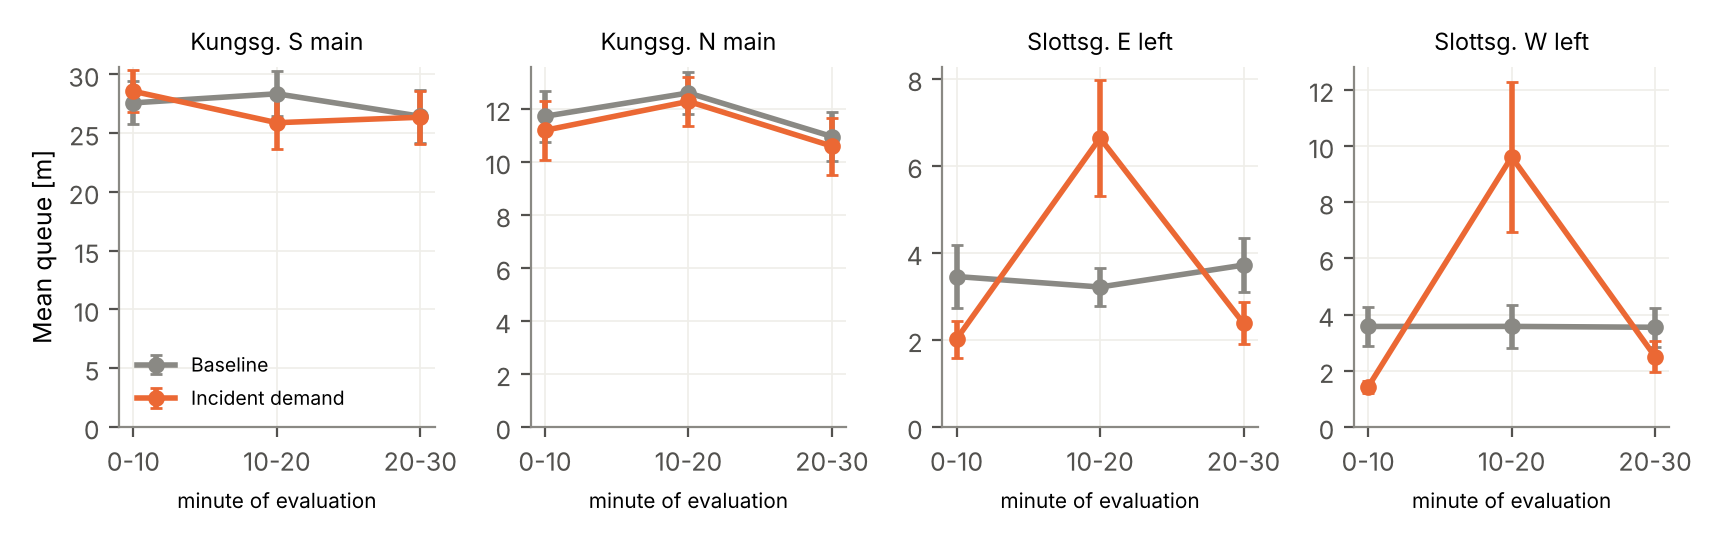
\includegraphics[width=0.95\textwidth]{fig_alt_incident.png}\\[6pt]
\begin{columns}[T]
\begin{column}{0.48\textwidth}
\small
Minutes 10 to 20: Slottsgatan left-turn queues double (east 3.2 $\rightarrow$ 6.6~m) and almost
triple (west 3.6 $\rightarrow$ 9.6~m).
\end{column}
\begin{column}{0.48\textwidth}
\small
Minutes 20 to 30: all queues back to baseline. The effect is \hl{invisible in 30-min averages}.
\end{column}
\end{columns}
\end{frame}

%---------------------------------------------------------------------
\begin{frame}{800 bicycles per hour: the right-turn conflict}
\begin{columns}[T]
\begin{column}{0.48\textwidth}
\footnotesize
\begin{tabular}{lrr}
\toprule
 & \textbf{Baseline} & \textbf{800 bikes/h}\\
\midrule
Car flow L4 [veh/h] & 943 & 878\\
Car flow L6 [veh/h] & 999 & 945\\
Stops [1/veh] & 0.74 & 1.51\\
Bicycle speed [km/h] & 17.9 & 16.5\\
Bicycle queue [m] & about 1 & about 10\\
\bottomrule
\end{tabular}
\end{column}
\begin{column}{0.48\textwidth}
\small
\begin{itemize}\setlength{\itemsep}{5pt}
  \item Right-turners from Kungsgatan yield to an almost continuous stream of cyclists
  \item Car throughput \hl{$-7\,\%$}, stops doubled
  \item Average delay (+1.2~s) understates the effect on cars
  \item Next steps: separate right-turn phase or leading bicycle interval
\end{itemize}
\end{column}
\end{columns}
\end{frame}

%=====================================================================
\section{Conclusions and discussion}
%=====================================================================

\begin{frame}{Conclusions}
\small
\begin{itemize}\setlength{\itemsep}{5pt}
  \item A fully automated chain (variant generation, COM batch runs, GP surrogates, Sobol
        sensitivity, constrained optimisation, validation) calibrated the model with 1\,857 runs
  \item Most influential: right-turn speed, desired speed per approach, acceleration and
        deceleration functions, bicycle desired speed; conflict-area gaps irrelevant
  \item Speed-only calibration gives an invalid model; accelerations must be a target
  \item Recommended model (phase 2): speed RMSE \hl{2.01~km/h}, acceleration RMSE 0.13~m/s$^2$,
        \hl{10/20} tests, all bicycle locations pass, demand served
  \item Remaining errors are structural (turning behaviour, one acceleration function)
  \item Actuated control: delay \hl{$-26\,\%$}; incident: temporary side-road queues only;
        800 bicycles/h: car throughput $-7\,\%$
\end{itemize}
\end{frame}

%---------------------------------------------------------------------
\begin{frame}{Questions for discussion}
\small
\begin{itemize}\setlength{\itemsep}{6pt}
  \item Speed-only fitting produced a model that was ``right for the wrong reason''. Should
        acceleration data be a standard calibration target?
  \item L1 has a field s.d.\ of 4.7~km/h but L3 only 0.3~km/h: an RMSE treats them equally, the
        $t$-test does not. Which acceptance criterion should a calibration use?
  \item Remaining misfits look structural. When should we change the model instead of its
        parameters?
  \item The actuated controller gains 26\,\% by taking green from the side road. Is average delay
        the right objective, or should side-road waiting be weighted?
  \item The model was calibrated at 100 bicycles/h, but the bicycle scenario depends on
        car-cyclist conflicts the data could not calibrate. How far can a calibrated model be
        extrapolated?
\end{itemize}
\end{frame}

%---------------------------------------------------------------------
\begin{frame}[plain]
\centering
\vfill
{\color{accent}\Huge\bfseries Thank you}\\[10pt]
{\large Questions?}\\[18pt]
\small Code, data, report and figures: private GitHub repository\\[2pt]
\texttt{vissim-surrogate-calibration}
\vfill
\end{frame}

\end{document}
